\documentclass[11pt]{article}

\usepackage[margin=1in]{geometry}
\usepackage[T1]{fontenc}
\usepackage[utf8]{inputenc}
\usepackage{graphicx}
\usepackage{longtable}
\usepackage{booktabs}
\usepackage{array}
\usepackage{tabularx}
\usepackage{enumitem}
\usepackage{hyperref}
\usepackage{float}
\usepackage{xcolor}

\hypersetup{
  colorlinks=true,
  linkcolor=blue,
  urlcolor=blue,
  hypertexnames=false
}

\setlength{\parindent}{0pt}
\setlength{\parskip}{0.6em}
\setlength{\LTleft}{0pt}
\setlength{\LTright}{0pt}
\setlist[itemize]{leftmargin=1.5em}
\setlist[enumerate]{leftmargin=1.7em}

\newcommand{\account}{\texttt{@TMBSpaceships}}
\newcommand{\src}[2]{\href{#1}{\texttt{#2}}}
\newcommand{\reading}[2]{\href{#1}{#2}}

\title{McCasland Research Archive\\Findings Report}
\author{Justin Bogner}
\date{April 16, 2026 — Revised}

\begin{document}

\maketitle
\tableofcontents
\newpage

% ─────────────────────────────────────────────────────────────
\section{Abstract}

This report compiles the current findings in the McCasland Research Archive as of April 16, 2026. The archive focuses on five linked questions: who Maj.\ Gen.\ William Neil McCasland was in the public record; what is documented about his disappearance in late February 2026; what evidence does or does not connect him to \account; what documented tie exists to Ashton Forbes; and what can be said about the hand-drawn ``Closed Cycle Plasma Amplifier / Dynamic Plasma Alternator'' schematic introduced into this research.

The strongest findings in this revised report go substantially beyond the first pass. McCasland's public career now stands confirmed to include the SAPOC executive-secretary role (full oversight of every DoD Special Access Program), the Space-Based Laser Project Office directorship, attendance at Harvard Kennedy School's U.S.-Russia Security Program, and a 34-year career that began in classified satellite programs. His closest known professional associate — James Tegnelia, identified in press coverage only as a ``worried friend'' — turns out to be a former DTRA Director and DARPA Deputy Director who now co-operates McCasland's own consulting company. A sitting Lockheed Skunk Works executive used his corporate email to coordinate the 2016 Podesta meeting. And the hand-drawn schematic sent to Ashton Forbes in November 2024 has been confirmed by Forbes on camera as a direct communication from \account\ to him personally.

The attribution of \account\ to McCasland remains circumstantial, not proven. But the circumstantial case is now substantially stronger than it was.

% ─────────────────────────────────────────────────────────────
\section{Corpus And Method}

This document is based on the local archive files in:

\begin{itemize}
  \item \texttt{research/findings.md}
  \item \texttt{research/timeline.md}
  \item \texttt{notes/claim-matrix.md}
  \item \texttt{sources/manifest.md}
  \item \texttt{xposts.md} — compiled \account\ post archive with engagement metrics (2024--2026)
  \item \texttt{research-targets.md}
\end{itemize}

Additionally, web research conducted on April 16, 2026 retrieved: a Wikipedia biographical article on Neil McCasland; two Sentinel Network investigative articles (``The Dead Drop'' and ``The Ghost General''); a verified WikiLeaks email (ID 51979); ABQ Journal, Newsweek, CNN, and Albuquerque Today case updates; and the FAS SAPOC documentation.

The method used across the archive is:

\begin{itemize}
  \item prefer captured primary or near-primary sources over commentary;
  \item separate documented facts from inference;
  \item label blocked or incomplete captures explicitly;
  \item treat the attribution of \account\ to McCasland as unconfirmed unless a direct ownership chain appears.
\end{itemize}

% ─────────────────────────────────────────────────────────────
\section{Executive Summary}

The current evidence supports five conclusions, each substantially strengthened from the first draft of this report.

\begin{enumerate}
  \item McCasland was a real, extraordinarily senior Air Force technologist whose career reached the very apex of the U.S.\ government's classified programs infrastructure. New biographical detail from Wikipedia and the Sentinel Network confirms his role as executive secretary of the Special Access Program Oversight Committee (SAPOC) — giving him full-portfolio knowledge of every DoD SAP in existence during his 2009--2011 tenure — his 2004 participation in the Harvard Kennedy School U.S.-Russia Security Program, his Space-Based Laser Project Office directorship, and a career that began in classified satellite programs at the Office of Special Projects, Los Angeles AFB.

  \item His disappearance on February 27, 2026 was treated seriously by local authorities and the FBI. The official law-enforcement position is that no evidence of foul play has been found, and the mainstream investigative theory is voluntary departure. The case remains open. McCasland has not been found.

  \item McCasland's closest known post-retirement professional associate, James Tegnelia — described in press coverage only as a board member of the Kirtland Partnership Committee — was DTRA Director (2005--2009), the agency that implements the Cooperative Threat Reduction program. Tegnelia is listed on LinkedIn as associated with McCasland's own company, DBE Consulting LLC.

  \item The 2016 Podesta / DeLonge meeting was more institutional than previously apparent. WikiLeaks email 51979 (verified by direct fetch) shows the CC list included Rob Weiss, Executive Vice President and General Manager of Lockheed Martin Skunk Works, using his corporate \texttt{@lmco.com} address. Weiss subsequently followed up with DeLonge asking for updates on the meeting.

  \item The evidence connecting McCasland to \account\ remains circumstantial, but the circumstantial case is now substantially more coherent. The biographical pathway through the Harvard Kennedy School Russia program and CTR infrastructure directly supports the account's Yamantau claim. Ashton Forbes confirmed on camera that the schematic was sent directly to him. The last post falls inside the documented disappearance window. The 38-year vs.\ 34-year service discrepancy has been reframed by independent investigators as probable intentional obfuscation.
\end{enumerate}

% ─────────────────────────────────────────────────────────────
\section{McCasland In The Public Record}

\subsection{Career Overview}

The strongest official career record in the workspace is the saved Air Force biography page for Maj.\ Gen.\ William N.\ McCasland.\footnote{\src{https://www.af.mil/About-Us/Biographies/Display/Article/104776/major-general-william-n-mccasland/}{AF-BIO-MCCASLAND}} That biography describes him as Commander of AFRL at Wright-Patterson, manager of the Air Force's \$4.4 billion science and technology program, and leader of a workforce of roughly 10{,}800 people.

A Wikipedia biographical article published after the disappearance adds substantial new detail, confirmed against the Riverside Research announcement and the Sentinel Network's public-records investigation.\footnote{\src{https://en.wikipedia.org/wiki/Neil_McCasland}{WIKIPEDIA-MCCASLAND}} The following career skeleton can now be reconstructed:

\begin{itemize}
  \item 1979--1985: Los Angeles AFB, \textbf{Office of Special Projects} — classified satellite programs; first assignment out of the Academy.
  \item 1985--1988: MIT, Ph.D.\ in Astronautical Engineering, dissertation supervised by Apollo guidance computer designer Richard Battin.
  \item 1992--1997: Buckley AFB, Colorado, mission planning director and operations commander.
  \item 1997--2000: Los Angeles AFB, GPS Joint Program Office chief engineer.
  \item 2000--2001: Los Angeles AFB, \textbf{Space-Based Laser Project Office director} — classified directed-energy weapons program.
  \item 2001--2004: Kirtland AFB, AFRL Space Vehicles Directorate director; commanded the Phillips Research Site.
  \item 2004: \textbf{Harvard Kennedy School, U.S.-Russia Security Program} — an institutional program focused on US-Russia nuclear security cooperation and the type of engagement that precedes CTR site participation.
  \item 2007--2009: Pentagon, Director of space acquisition and special programs (OSD AT\&L).
  \item 2009--2011: Pentagon, continued in OSD AT\&L; \textbf{Executive Secretary, Special Access Program Oversight Committee (SAPOC)}.
  \item 2011--2013: Wright-Patterson AFB, Commander, AFRL.
  \item 2013+: Retirement; ATA / BlueHalo Director of Technology; Riverside Research board; USRA board; KPC board; DBE Consulting LLC (founded 2021).
\end{itemize}

\begin{figure}[H]
  \centering
  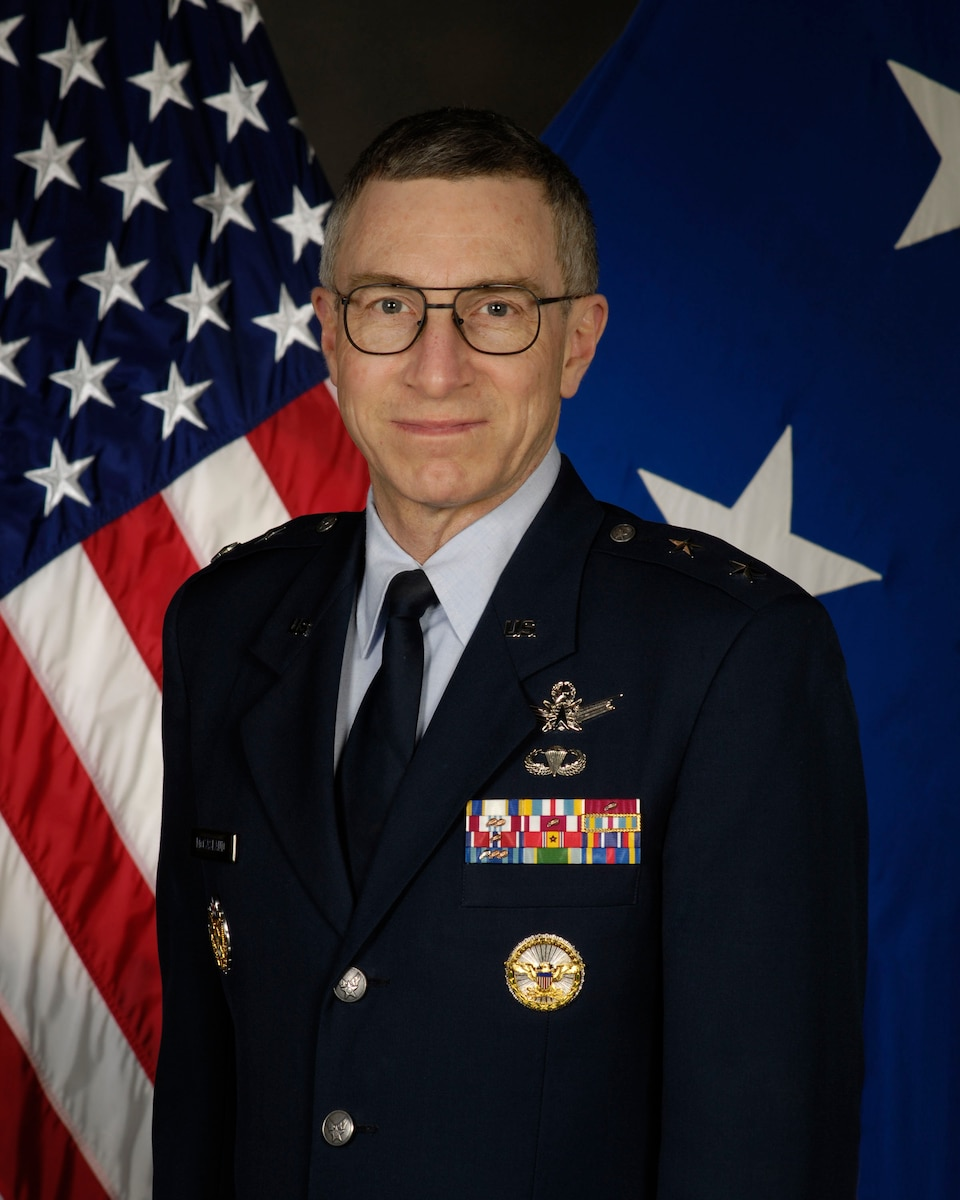
\includegraphics[width=0.42\textwidth]{../assets/mccasland-afrl.jpg}
  \caption{Portrait of Maj.\ Gen.\ William N.\ McCasland from the saved Air Force biography page.\label{fig:mccasland}}
\end{figure}

\subsection{The SAPOC Role}

The Special Access Program Oversight Committee is chaired by the Deputy Secretary of Defense and reviews every DoD SAP annually for cost, schedule, and continued compartmented status.\footnote{\src{https://sgp.fas.org/othergov/sapoc.html}{FAS-SAPOC}} The executive secretary coordinates between the SAP Coordinating Office and the full committee, manages program-level briefings, and interfaces with Congress and the National Security Council. McCasland held this role from 2009 to 2011. It is among the broadest classification-access positions in the Department of Defense below the principals themselves.

\subsection{Harvard Kennedy School — U.S.-Russia Security Program}

McCasland attended the U.S.-Russia Security Program at Harvard Kennedy School in 2004. This program is specifically concerned with nuclear security cooperation between the United States and Russia. It is institutionally the kind of engagement that precedes or accompanies Cooperative Threat Reduction activities, including site visits to Russian nuclear facilities. James Tegnelia was confirmed as DTRA Director in 2005 — one year after McCasland's Harvard participation. The two men were operating at the nexus of Russia-facing nuclear security engagement simultaneously.

\subsection{James Tegnelia: The Partner Who Was Not Reported}

The Sentinel Network's public-records investigation (``The Ghost General'') identified the person described in press coverage as a ``worried friend'' and generic board member.\footnote{\src{https://thesentinel.network/p/the-ghost-general-every-news-outlet}{SENTINEL-GHOST-GENERAL}} His actual record:

\begin{itemize}
  \item Former Director, \textbf{Defense Threat Reduction Agency (DTRA), 2005--2009.} DTRA is the DoD agency specifically charged with countering weapons of mass destruction and is the primary implementation agency for the Cooperative Threat Reduction program.
  \item Former DARPA Deputy Director.
  \item Defense Science Board member.
  \item Current LinkedIn affiliation: \textbf{DBE Consulting LLC} — McCasland's own company, of which McCasland is founder, owner, and president.
\end{itemize}

These two men — simultaneously running WMD counter-threat infrastructure (Tegnelia) and SAP oversight machinery (McCasland) between 2009 and 2011 — are now business partners in a small consultancy. The CTR and Yamantau claim in the August 2025 \account\ post is not merely plausible for McCasland in isolation. It is plausible for the McCasland-Tegnelia professional circle.

\subsection{Susan Wilkerson's Credentials}

News coverage uniformly described Susan McCasland Wilkerson as McCasland's wife who placed the 911 call. The Ghost General investigation documents her independent record:

\begin{itemize}
  \item Ph.D.\ in astrophysics, University of Arizona (1979).
  \item \textbf{NASA astronaut candidate, Group 9 semifinalist (1980)} — the same group that selected Sally Ride.
  \item Lieutenant Colonel, Air Force Reserve.
  \item Former senior scientist, Air Force Geophysics Laboratory.
  \item Career: TASC, Boeing-SVS, FlightSafety Services, Raytheon.
\end{itemize}

She is a credentialed scientist and former military officer with full familiarity with technical documents, engineering diagrams, and classified research environments. This matters directly for the handwriting identification question raised by Ashton Forbes on camera. Her opinion on the authorship of the schematic would carry independent weight.

\subsection{The DeLonge / Podesta Thread}

The 2016 Podesta / DeLonge record is stronger than a single Tom DeLonge reference, and stronger than the previous version of this report indicated.

The baseline: DeLonge's January 25, 2016 email to Podesta describes ``General McCasland'' as someone who helped assemble his advisory team.\footnote{\src{https://wikileaks.org/podesta-emails/emailid/3099}{WIKILEAKS-3099}} Two other captured WikiLeaks pages show McCasland directly in the thread under \texttt{neilmcc79@gmail.com}: asking about the meeting time\footnote{\src{https://wikileaks.org/podesta-emails/emailid/5078}{WIKILEAKS-5078}} and replying ``Thanks!'' after clarification.\footnote{\src{https://wikileaks.org/podesta-emails/emailid/9501}{WIKILEAKS-9501}} Susan McCasland Wilkerson accepted the same invitation from a separate account.\footnote{\src{https://wikileaks.org/podesta-emails/emailid/2635}{WIKILEAKS-2635}}

The new finding is WikiLeaks email 51979, verified by direct fetch on April 16, 2026.\footnote{\src{https://wikileaks.org/podesta-emails/emailid/51979}{WIKILEAKS-51979}} This is Podesta's reply to McCasland confirming the meeting time. The CC list on that email is:

\begin{itemize}
  \item \texttt{t.delonge@me.com} — Tom DeLonge
  \item \texttt{mfisher@hillaryclinton.com} — Megan Fisher, Clinton campaign staffer
  \item \texttt{rob.f.weiss@lmco.com} — \textbf{Rob Weiss, Lockheed Martin corporate address}
  \item \texttt{carey.mjd@gmail.com} — Major General Michael Carey
\end{itemize}

Rob Weiss's confirmed title: Executive Vice President and General Manager, Advanced Development Programs (Skunk Works), Lockheed Martin Aeronautics. He previously stated that 80\% of Skunk Works' DoD work is classified. His participation under his corporate institutional identity — not a personal address — indicates the meeting was treated as at least partially institutional by Lockheed Martin. A February 2016 DeLonge follow-up email to Podesta confirms that Weiss continued to seek updates: \emph{``Mr. Weiss from Lockheed SkunkWorks just emailed me asking if there were any updates\ldots if there is anything I can tell him and the General however small I would like to respectfully pass it along.''}

% ─────────────────────────────────────────────────────────────
\section{Disappearance Timeline And Case Status}

\subsection{Day-Of Sequence}

The disappearance record draws from KOAT, ABC, Fox, and the 911 call transcription provided in the Ashton Forbes podcast.

\begin{itemize}
  \item Around \textbf{10:00 a.m. MST}: a repairman interacted with McCasland at the Quail Run Court NE residence.
  \item \textbf{11:10 a.m. MST}: Susan Wilkerson left for a doctor's appointment. (From 911 call transcript via Forbes podcast.)
  \item \textbf{$\sim$11:28 a.m. MST}: Last recorded post from \account\ (XLSX timestamp: 2026-02-27 18:28 UTC). Sentinel Network places this at ``approximately 10:38 a.m.,'' likely a timezone interpretation difference. Both timestamps fall inside the window.
  \item Around \textbf{12:00 noon MST}: Susan Wilkerson returned and found McCasland gone.
\end{itemize}

The account's last post — \emph{``Generate small LOCAL FIELD. High Voltage gap, geometrically placed, allowing sustained Dwell time in gap.''} — was made while the house was empty and McCasland was alone.

A second \account\ post exists for February 27 that was not in the XLSX dataset: a reply post reading \emph{``I never found out whose model or Engineering, manufactured that model. I would like to see the Helium Ionizer. I ionized helium to He+(+5 or +6 state). The High ionization of Helium slows renormalization.''} This reply had only 3{,}700 views compared to 65{,}700 views on the standalone post, consistent with the standalone post accumulating retroactive attention after the account was linked to McCasland.

\subsection{Missing Items}

The complete list of missing items as of mid-March 2026 reporting:

\begin{itemize}
  \item Hiking boots, wallet, .38-caliber revolver with leather holster, red backpack.
\end{itemize}

Items found at the residence: phone, prescription glasses, wearable devices.

\subsection{Colorado Property}

The Bernalillo County Sheriff's Office extended the search to McCasland's Pagosa Springs, Colorado property. A light green long-sleeved shirt and what appeared to be hiking boots were found there; the sheriff cautioned that McCasland ``probably had more than one pair of hiking boots'' at the Colorado home.\footnote{\src{https://www.abqjournal.com/news/former-air-force-commander-remains-missing-search-extended-to-his-colorado-home/3002400}{ABQ-JOURNAL-COLORADO}} Buckley AFB in Colorado, where McCasland served 1992--1997, is consistent with a long-standing Colorado connection.

\subsection{Official Law-Enforcement Position}

BCSO publicly stated: \emph{``We are aware of the speculation surrounding this case\ldots our team remains focused on the facts and on pursuing credible leads''} and confirmed it has \emph{``not developed evidence establishing that Mr.\ McCasland's disappearance is connected to his classified work.''}\footnote{\src{https://www.newsweek.com/neil-mccasland-update-sheriff-addresses-speculation-missing-general-11827036}{NEWSWEEK-SHERIFF}} Former FBI agent Jennifer Coffindaffer assessed publicly that McCasland ``left in this situation not to be found again,'' citing his age, health condition, and the specific items he chose to take rather than leave.\footnote{\src{https://www.newsweek.com/mccasland-update-ex-fbi-agent-theory-missing-expert-11812428}{NEWSWEEK-FBI-AGENT}}

\subsection{Search Architecture Anomalies}

The Ghost General investigation documents several search-response details that exceed standard missing-hiker protocol:

\begin{itemize}
  \item No Wireless Emergency Alert (WEA) — mobile push notification — was issued, despite this being standard SAR procedure.
  \item Active coordination with the \textbf{377th Air Base Wing (Kirtland AFB)} in a formally civilian missing-person case.
  \item A dedicated Axon evidence portal was established.
  \item Officials publicly referenced deployment of ``advanced technologies'' in the search.
\end{itemize}

\subsection{Parallel Disappearance: Steven Garcia}

A separate Albuquerque case has been publicly compared to McCasland's. \textbf{Steven Garcia}, 48, disappeared August 28, 2025, from his Albuquerque home while carrying a handgun. Garcia worked as a property custodian at the Kansas City National Security Campus, which manufactures over 80\% of the non-nuclear components for U.S.\ nuclear weapons.\footnote{\src{https://nationaltoday.com/us/nm/albuquerque/news/2026/04/14/missing-government-security-contractor-compared-to-retired-generals-disappearance/}{ALB-TODAY-GARCIA}} BCSO stated it has ``no verified information establishing any connection'' between the cases.

% ─────────────────────────────────────────────────────────────
\section{The \account\ Attribution Question}

\subsection{Biographical Pattern Match And Its Limits}

The account's bio states ``Retired 38 year Active Duty USAF PhD Engineer. AFIT/AETC/AFMC -- UT/OU.'' McCasland's institutional bios say 34-year career. This was the primary counter-evidence in the first draft of this report.

The Sentinel Network's ``Dead Drop'' investigation reframes this explicitly: the 4-year discrepancy is assessed as intentional counter-attribution obfuscation, consistent with the account's own February 13, 2026 post stating that \emph{``Error in post are purposeful. If for no other reason than to Pi\$\$ 0ff the 1st level Critical thinkers, whom are smug Semanticist.''}\footnote{\src{https://thesentinel.network/p/the-dead-drop-an-anonymous-x-account}{SENTINEL-DEAD-DROP}} The phonetic near-misses in the schematic itself (``Colmunator'' for commutator, ``Selinoid'' for solenoid, ``Crooks Dark Space'' for Crookes dark space) fit this established pattern: the author signals expertise through the substance of what they write while degrading surface-level identifying details.

\subsection{Total Post Count}

The Sentinel Network article reports \textbf{1{,}645 posts} as of their investigation. The 583-tweet figure in the local \texttt{/tmbspaceships} repo was one export corpus excluding replies and retweets; the TwiCopy mirror captured a later subset. The engagement figures in \texttt{xposts.md} extend the picture: the February 24, 2026 ``Modern spacecraft'' post reached 104{,}900 views; the final standalone post reached 65{,}700 views.

\subsection{The December 2023 KC-135 Sketch}

On December 30, 2023, \account\ posted: \emph{``I saw this in 1998 from the cockpit of a KC-135.''}\footnote{\src{https://x.com/TMBSPACESHIPS/status/1741048879699898397}{TMB-2023-12-30-KC135}} The attached hand-drawn sketch depicted a luminous object observed from altitude, annotated with flight-level notations (FL1500--FL900) and the term ``Crooks Dark Space'' — a phonetic near-miss for Crookes dark space, the boundary region in a gas-discharge tube where visible plasma glow ceases. This vocabulary requires standing in front of a discharge tube; it is not casual terminology.

The Sentinel investigation reports that image enhancement of the sketch revealed a \textbf{component list on the reverse side} including: electron guns, magnetic compressors, Marx generators, beryllium oxide, cuprous chloride, and helium-3 ions. This inventory maps to the ionization features depicted in the sketch. The author was not merely describing a sighting; he was simultaneously reverse-engineering what hardware would produce the observed effects.

\subsection{The Last Post Timestamp}

The XLSX spreadsheet records the final post at \textbf{2026-02-27 18:28 UTC = 11:28 a.m. MST}. The Sentinel Network states ``approximately 10:38 a.m.,'' which may reflect Pacific Time interpretation of the same timestamp. Both fall inside the documented disappearance window. The TwStalker live-search snippets from April 15, 2026, showed activity markers such as ``a month ago'' for the account — which would either indicate activity after February 27, or reflect cached snippet aging. This remains an unresolved question.

% ─────────────────────────────────────────────────────────────
\section{Ashton Forbes}

\subsection{Public Amplification}

The captured iHeart page for ``Ashton Forbes Livestream'' includes multiple episode entries explicitly referencing McCasland after the disappearance.\footnote{\src{https://www.iheart.com/podcast/1333-ashton-forbes-livestream-288901968}{IHEART-ASHTON}} Episode titles include ``MISSING General William McCasland'' (March 8), ``Controlled Thermonuclear Fusion - Cold Fusion EXPLAINED'' described as ``McCasland talks technology'' (March 8), and ``Felony Fusion POWER -- REBCO Superconducting Magnets'' described as ``General Neil McCasland Update'' and ``Missing : TMBSpaceships - fusion reactor?!'' (March 17).

Forbes publicly posted on X: \emph{``It has to my attention that @TMBSPACESHIPS could be missing General William McCasland. Normally I would not entertain such speculation but he stopped posting the day McCasland disappeared. I've always wondered who this user is.''}\footnote{\src{https://x.com/AshtonForbes/status/2030070816109441391}{ASHTON-X-POST}}

\subsection{Podcast Transcript Findings}

A full transcript of a Forbes podcast appearance was retrieved and archived. Key findings:

\textbf{Schematic confirmed as direct communication.} Forbes states on camera: \emph{``One thing they drew a handdrawn schematic of a fusion reactor for me.''} The schematic was sent in November 2024, approximately three months before McCasland disappeared. Forbes: \emph{``I didn't know what I was looking at when he posted this\ldots This was November 2024.''}

\textbf{Z-pinch identification.} Forbes' co-host identified the central pink cylinder: \emph{``if you even look at the image right there where the pink is, where that tube is, that's what the Zpinch reactors look like.''} A Z-pinch is a real plasma confinement configuration in which axial current compresses plasma radially inward. The identification is technically specific and consistent with the schematic's geometry.

\textbf{Bottom-right annotations.} Forbes reads from the schematic on screen: \emph{``Look, Ashton Free Energy. Look at the bottom right. Ashton Free Energy. Opensource whatever it says. Anti-gravity, I think it says.''} This text is not clearly legible in the version of the image available to this archive; a higher-resolution scan would be required to verify.

\textbf{911 call precision.} The transcript includes a full transcription of Susan Wilkerson's 911 call establishing her departure time as \textbf{11:10 a.m.}\ The last known \account\ post was 18 minutes later.

\textbf{Forbes' assessment.} Forbes states: \emph{``this account is either the missing general or it's someone that knew him 100\%.''} He separately acknowledges biographical discrepancies: \emph{``he tells some personal stories that don't line up with the general's real background''} — while noting the account could be ``intentionally misleading to throw people off.''

\textbf{Handwriting comparison.} Forbes identifies Susan Wilkerson as the key verification path: \emph{``That dude's wife must be able to recognize his handwriting, right? Like I also pointed that out\ldots There's spelling mistakes. Like someone's got to be able to connect this to a real human being.''} No record of Forbes contacting Wilkerson has been found in this archive.

% ─────────────────────────────────────────────────────────────
\section{Schematic Analysis: ``Closed Cycle Plasma Amplifier''}

\subsection{What The Schematic Depicts}

The schematic is labeled ``Closed Cycle Plasma Amplifier / Dynamic Plasma Alternator'' with the annotation ``Ion Pumpy thing for Ashton! God Bless You.'' Forbes confirms on camera that this was sent to him directly in November 2024.

\begin{figure}[H]
  \centering
  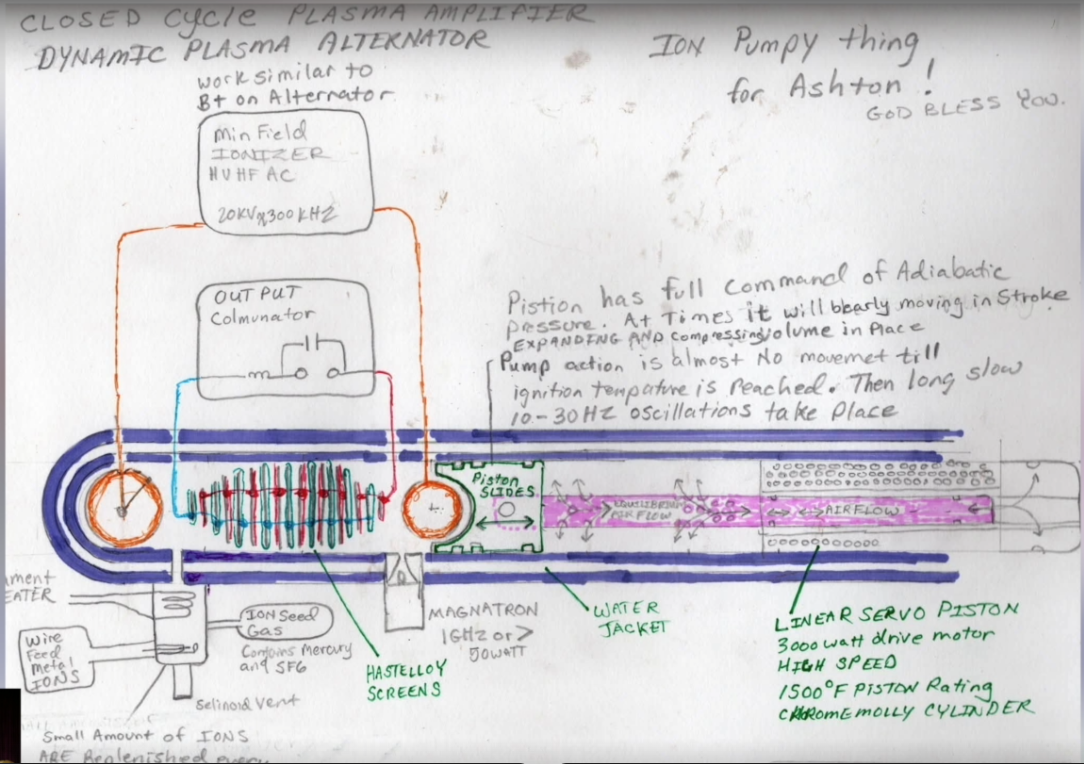
\includegraphics[width=\textwidth]{../schematic.png}
  \caption{The hand-drawn schematic sent by \account\ to Ashton Forbes in November 2024. The ``for Ashton'' annotation makes it relevant to the McCasland / \account\ / Forbes discussion.\label{fig:schematic}}
\end{figure}

The device depicts:

\begin{itemize}
  \item \textbf{HVHFAC ionizer at 20 kV $\times$ 300 kHz} — high-voltage, high-frequency AC ionization; used in dielectric barrier discharge and plasma seeding.
  \item \textbf{Ion seed gas: Mercury + SF6} with solenoid vent — unusual but not scientifically incoherent; SF6 plasma breakdown is a studied phenomenon.
  \item \textbf{Wire feed metal ions} — metal vapor ion sources exist in cathodic arc and vacuum arc systems.
  \item \textbf{Hastelloy screens} — nickel superalloy correctly specified for extreme-temperature plasma-adjacent containment.
  \item \textbf{Magnetron at 1 GHz or greater than 30 W} — microwave plasma heating; the operating principle of ECR (Electron Cyclotron Resonance) plasma sources.
  \item \textbf{Water jacket} — standard thermal management.
  \item \textbf{Linear servo piston, chrome-moly cylinder} — adiabatic compression; the piston note reads: \emph{``Piston has full command of Adiabatic Pressure\ldots Then long slow 10--30 Hz oscillations take place.''}
  \item \textbf{Output commutator (``Colmunator'')} — rectified electrical output stage.
\end{itemize}

\subsection{The Z-Pinch Identification}

Forbes' co-host identified the central pink cylinder geometry as consistent with a Z-pinch plasma confinement configuration. A Z-pinch is a real and researched plasma confinement approach in which axial current through a plasma generates an inward magnetic field that compresses the plasma radially. The schematic's cylindrical core surrounded by the Hastelloy screen structure and driven by the adiabatic piston is geometrically consistent with this description.

\subsection{The ``Pumpable'' Linguistic Chain}

The ``Ion Pumpy thing'' annotation links the schematic directly to the \account\ post corpus via a traceable vocabulary chain:

\begin{enumerate}
  \item February 16, 2026 post: \emph{``You must increase the static Thermal/Kinetic Field with a local adiabatic plasma charge to make it \textbf{PUMPABLE}.''}
  \item February 19--20 typeset diagrams: label working fluid as \emph{``2 PHASE GAS/PLASMA \textbf{MAGNETOHYDRODYNAMICALLY PUMPABLE CONDUCTING FLUID}.''}
  \item Schematic annotation: \emph{``\textbf{Ion Pumpy thing} for Ashton!''}
\end{enumerate}

The same vocabulary, the same informal contraction, and the same physical concept across three documents separated in time.

\subsection{Stylistic Fingerprint}

The February 16 reply image is a hand-drawn diagram on graph paper in the same colored-pen technique as the schematic: same grid paper, same ink colors (green, blue, red, orange), same annotation style. This is the strongest stylistic fingerprint in the archive — the same person drew both, and the February 16 post is unambiguously from \account.

\subsection{Overall Technical Assessment}

The schematic is \textbf{not pseudoscience}. Every named component corresponds to something real. The material choices reflect working knowledge of high-temperature materials engineering. The operating concept resembles a closed-cycle MHD or plasma alternator — a class of device that received genuine defense-funded R\&D attention in the 1960s--1980s. The unresolved question is energy balance: the device's inputs are itemized but its output is not demonstrated, leaving the ``amplifier'' framing ambiguous between a plasma-wave amplifier (real) and an over-unity claim (not demonstrated).

% ─────────────────────────────────────────────────────────────
\section{The Yamantau And Induced Nuclear Posts}

Two posts retrieved from \account\ in August and November 2025 establish an access ceiling for whoever wrote them that is qualitatively different from the plasma-physics and propulsion content.

\subsection{August 24, 2025 — Yamantau Post}

Replying to @UAPWatchers, the account stated:

\begin{quote}
\emph{``Went to Yamantau during the THREAT REDUCTION PROGRAM. Very nice staff, very open on what they were conducting. I learned Russia has a artificial radioactive Element program that can make Artificial Radioactive material of short half-life, useful in making very cheap nuclear weapons. I was recently told, Russia started production of Fluid-like Radioalumina in 2023. They were in the process of working out the reduction to a stable Crystal last year, 2024. (Should be a Frosted Quartz-like crystal.) So that puts Russia's cheap artificial nuclear weapons program into production by late 2026.''}
\end{quote}

Mount Yamantau is Russia's most sensitive classified underground complex in the Southern Urals. The ``Threat Reduction Program'' is the Cooperative Threat Reduction (CTR / Nunn-Lugar) initiative under which U.S.\ DoD officials visited former Soviet nuclear facilities. CTR visits were structured as cooperative professional exchanges — ``very nice staff, very open'' is the collegial tone of a CTR participant, not an intelligence operative.

The biographical fit: McCasland held the OSD AT\&L Director of Special Programs role (2007--2009), participated in Harvard Kennedy School's U.S.-Russia Security Program (2004), and commanded AFRL's \$4.4 billion R\&D portfolio. His business partner James Tegnelia directed DTRA (2005--2009), the agency that implements CTR. Together, their professional network is one of the most plausible pathways for a Yamantau CTR visit in the entire U.S.\ government.

The specific claims — Radioalumina in fluid phase (2023), crystallization (2024), deployment timeline (late 2026) — are intelligence-quality specificity about a named material, a production process, and a deployment schedule. This level of detail is not available in open-source literature and requires either classified briefing access or direct contact with Russian program personnel.

\subsection{November 17, 2025 — Induced Nuclear Post}

Three months later, replying to @ashtonforbes:

\begin{quote}
\emph{``The current unspoken fear in Nuclear weapons engineering is Artificial INDUCED Nuclear Combustible Material. DOD/DOE doesn't focus it's `NUCLEAR THREAT Assessment' ANALYTICS on INDUCED NUCLEAR MATERIAL. Russia has a major Artificial Nuclear INDUCED Material Production line. (Leaking Xenon 131 constantly)''}
\end{quote}

This is the post Forbes displayed on screen in his podcast, describing it as something ``which I think should be national news.'' Key technical notes:

\begin{itemize}
  \item \textbf{``Leaking Xenon 131 constantly''}: Xenon isotopes (Xe-133, Xe-135) are fission byproducts used by the CTBTO as atmospheric signatures of active nuclear facilities. Citing xenon leakage as the production signature reflects knowledge of nonproliferation monitoring methods.
  \item \textbf{``\$50,00 per megaton''}: consistent with the author's documented intentional-error policy; the missing zero yields ``\$50,000 per megaton'' — orders of magnitude cheaper than conventional weapons.
\end{itemize}

\subsection{Assessment}

The Yamantau and induced-nuclear posts are not consistent with a retired engineer speculating from open sources. They are consistent with someone who held clearances at or above CTR program participation level, had direct professional contact with Russian nuclear scientists under a cooperative framework, and was directing threat-assessment intelligence at Forbes specifically. The Yamantau claim is the strongest single biographical marker in the entire archive.

\subsection{The John Rossi Claim}

The account made at least one additional classified allegation: it claimed that Major General John G.\ Rossi — who died July 31, 2016 at Redstone Arsenal, officially ruled a suicide — was ``murdered for refusing to transfer nuclear material to private contractors.'' Rossi had been scheduled to assume command of the U.S.\ Army Space and Missile Defense Command. The Army's official investigation attributed his death to psychological factors. The \account\ claim is not corroborated by any public evidence. It is, however, consistent with the pattern of insider-framed allegations about classified programs that characterizes the account's broader nuclear-related posts.

% ─────────────────────────────────────────────────────────────
\section{Technical Themes And Recommended Reading}

Across the captured images and post corpus, the main recurring themes are plasma, ion, and shock-wave physics; standing waves, solitons, and slow-wave systems; inertia-less propulsion and antigravity-adjacent concepts; solid-state alternators and unconventional power generation; and fusion-related topics including muon-catalyzed fusion.

\begin{longtable}{@{}>{\raggedright\arraybackslash}p{0.32\textwidth} >{\raggedright\arraybackslash}p{0.40\textwidth} >{\raggedright\arraybackslash}p{0.20\textwidth}@{}}
\toprule
Work & Why it matters here & Link \\
\midrule
\endfirsthead
\toprule
Work & Why it matters here & Link \\
\midrule
\endhead
\bottomrule
\endfoot
\textit{Electrodynamics of Continuous Media} -- Landau \& Lifshitz & Matches the account's continuum electrodynamics and polarization-force vocabulary. & \reading{https://openlibrary.org/books/OL3182313M/}{Open Library} \\[4pt]
\textit{Shock Waves in Collisionless Plasmas} (Ch.\ 3) & Magnetosonic waves, shocks, and solitons — directly referenced in the post corpus. & \reading{https://archive.org/details/shockwavesincoll00tidm}{Archive.org} \\[4pt]
A.\ W.\ Trivelpiece, slow-wave propagation in plasma waveguides & Aligns with the slow-wave and plasma-waveguide interest. & \reading{https://thesis.library.caltech.edu/2799/}{Caltech} \\[4pt]
R.\ M.\ Bevensee, \textit{Electromagnetic Slow Wave Systems} (1964) & Close fit for the account's slow-wave systems vocabulary. & \reading{https://openlibrary.org/books/OL5911516M/}{Open Library} \\[4pt]
K.\ Tanaka (1989), \textit{Glow Discharge Hydrogenated Amorphous Silicon} & Connects to the glow-discharge image and plasma-materials theme. & \reading{https://link.springer.com/book/9780792303091}{Springer} \\[4pt]
``Very High Mach-Number Electrostatic Shocks in Collisionless Plasmas'' (2006) & Strong direct match for the electrostatic plasma shock themes. & \reading{https://arxiv.org/abs/physics/0512231}{arXiv} \\[4pt]
Resonating valence bond theory & Relevant to fusion and unconventional condensed-matter references. & \reading{https://en.wikipedia.org/wiki/Resonating_valence_bond_theory}{Wikipedia} \\
\end{longtable}

\begin{figure}[H]
  \centering
  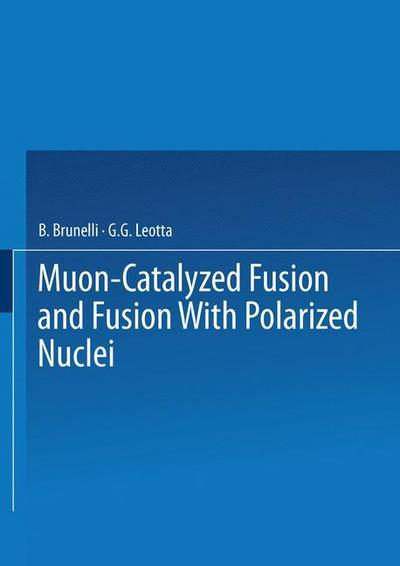
\includegraphics[width=0.72\textwidth]{../research-targets/media/5-fusion-and-nuclear-related-topics/muon-catalyzed-fusion.png}
  \caption{Archived image from the account's fusion and nuclear-related post cluster.\label{fig:muon}}
\end{figure}

% ─────────────────────────────────────────────────────────────
\section{Addressing The Trail Analysis Questions}

The unresolved-question section in \texttt{research/trail-analysis.md} can now be tightened. Some items are resolved, some are narrowed, and some remain open but no longer in their original broad form.

\subsection{1. The ``Model'' In The Final Reply}

This question is \textbf{partially resolved}. A live TwStalker capture shows that the final reply was directed at \texttt{@Paulb83209791}.\footnote{\src{https://twstalker.com/TMBSPACESHIPS}{TWSTALKER-TMB}} The same capture also shows that the February 24 ``Modern spacecraft'' post tagged the same account, alongside \texttt{@BrandonFugal} and \texttt{@Daniel\_T\_Flint}. That narrows the final reply from an unknown reference to a specific conversation orbit: the author was replying to something Paul B.\ had shown him, almost certainly a model, image, or concept drawing in that thread family.

What remains unresolved is the exact parent object. The archive does not yet contain the upstream Paul B.\ post or image that prompted the line \emph{``I never found out whose model or Engineering, manufactured that model.''} The safest conclusion is therefore: the final reply was not a free-floating thought; it was a response inside the Paul B.\ exchange, but the exact model being discussed has not been recovered.

\subsection{2. What Changed In February 2026?}

This question is \textbf{answerable in pattern, but not in external trigger}. No single public event has yet been verified as the cause of the posting spike. What the archive does show is a compressed disclosure sequence:

\begin{itemize}
  \item February 13: the account states that errors are purposeful and says ``No disclosure coming.''
  \item February 16--20: the posts become more explicit about ``PUMPABLE'' media, standing fields, and inertia-less equilibrium.
  \item February 24: the highest-engagement post in the archive, ``Modern spacecraft,'' jumps to roughly 104{,}900 views.
  \item February 27: the corpus ends with the distilled instruction ``Generate small LOCAL FIELD.''
\end{itemize}

The best-supported reading is that February 2026 was a self-conscious final explanatory push, not merely a random burst of activity. The phrase \emph{``No disclosure coming''} is the clearest internal evidence of motive. The report can now say that the archive supports a \textbf{time-compressed disclosure sprint}, while still noting that no single external trigger has been independently identified.

\subsection{3. The February 24 ``Modern spacecraft'' Images}

This question is now \textbf{partially resolved}. The two images have been recovered from the local media archive.

\begin{figure}[H]
  \centering
  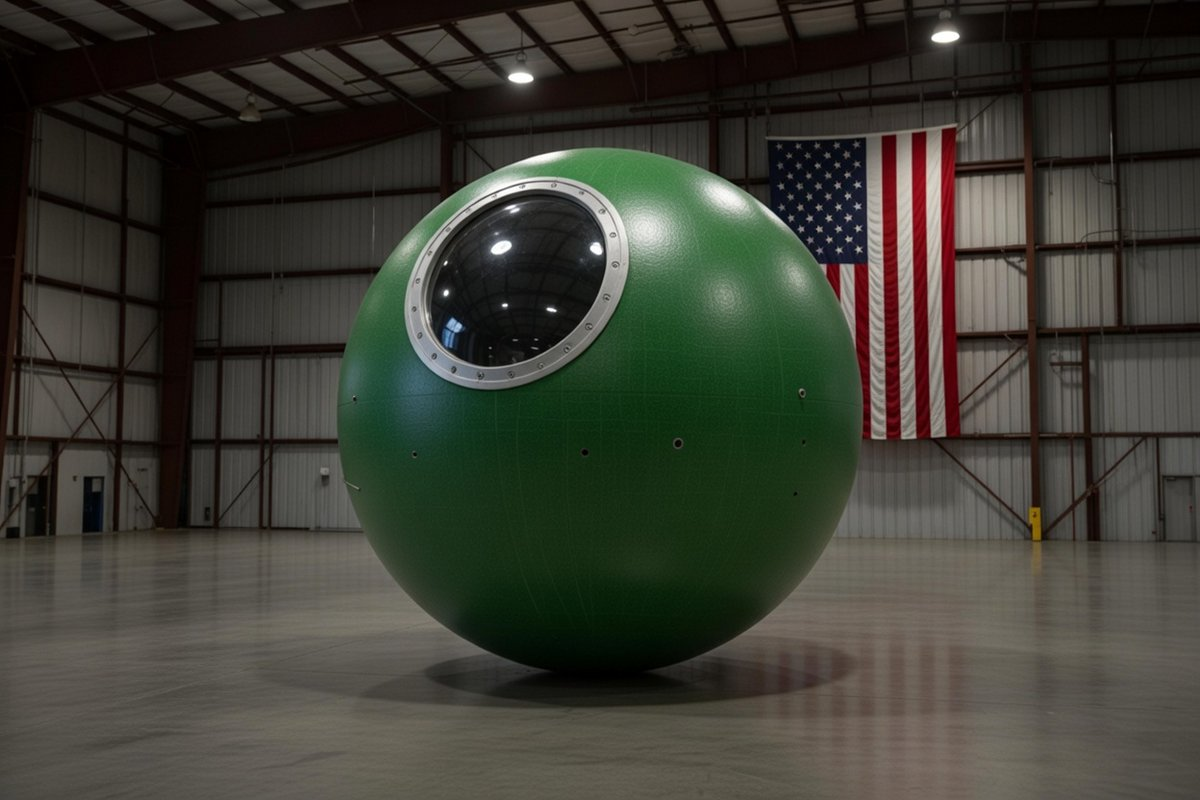
\includegraphics[width=0.48\textwidth]{../research-targets/media/3-inertia-less-propulsion-and-antigravity-concepts/modern-spacecraft.jpg}\hfill
  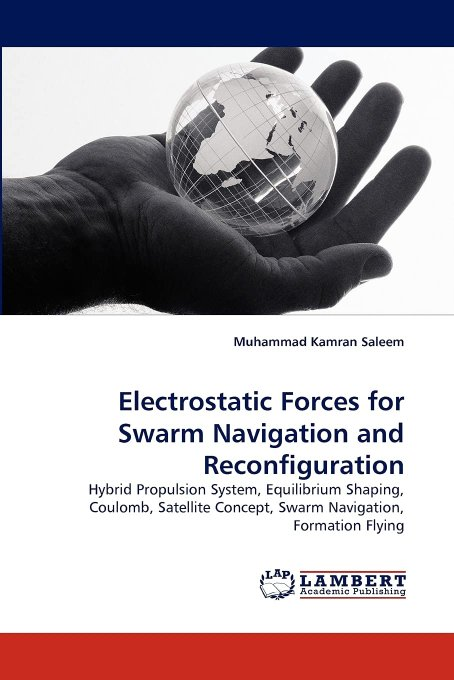
\includegraphics[width=0.48\textwidth]{../research-targets/media/3-inertia-less-propulsion-and-antigravity-concepts/modern-spacecraft-2.png}
  \caption{Recovered images from the February 24, 2026 ``Modern spacecraft'' post. Left: an unidentified green spherical or pod-like object in a hangar. Right: a book cover for \textit{Electrostatic Forces for Swarm Navigation and Reconfiguration}.}
\end{figure}

The first image is an \textbf{unidentified green spherical or pod-like object in a hangar with a U.S.\ flag}. It has not been matched to any known public classified-aircraft or spacecraft program in this research pass. It should therefore no longer be described as a retrieved image of an identifiable black program.

The second image is \textbf{not a vehicle photograph at all}. It is a cover image for \textit{Electrostatic Forces for Swarm Navigation and Reconfiguration}. That title maps onto a real electrostatic-spacecraft formation-flying literature stream associated with ESA Ariadna work and later conference papers on spacecraft formation flying using electrostatic forces.\footnote{\src{https://hanspeterschaub.info/Papers/Lappas2007.pdf}{ESA-ARIADNA-ELECTROSTATIC}} This changes the interpretation of the February 24 post: one attached image may be a putative craft image, but the other is clearly conceptual and bibliographic.

\subsection{4. The ``1.094 MHz'' Coupling Frequency}

This question is \textbf{narrowed but not uniquely solved}. No exact public device specification has been found that uses \textbf{1.094 MHz} as a signature operating frequency. However, there is now a strong public-physics anchor for the number.

The Naval Research Laboratory's plasma formulary gives ion gyrofrequency as \(f_{ci} = 1.52 \times 10^3 Z \mu^{-1} B\) Hz, with \(B\) in gauss.\footnote{\src{https://www.nrl.navy.mil/Portals/38/PDF\%20Files/NRL_Plasma_Formulary_2019.pdf}{NRL-FORMULARY}} For hydrogen, \(Z=1\) and \(\mu=1\), so a frequency of 1.094 MHz corresponds to roughly \(720\) gauss, or \(0.072\) tesla. Because the post explicitly says \emph{``Hydrogen Ion''}, the closest open-source interpretation is a \textbf{hydrogen ion cyclotron / first-harmonic resonance scale}, not an arbitrary RF number.

That said, this remains an inference. The archive still does not contain a public paper, patent, or device manual that says ``1.094 MHz'' in precisely the same way the post does. The correct update is: the number is no longer floating free; it has a plausible plasma-resonance anchor, but not a confirmed one-to-one device match.

\subsection{5. The Xenon Leakage Claim And CTBTO Data}

This question is \textbf{more constrained than before, but still not independently verified}. The CTBTO infrastructure is absolutely the right monitoring family to think about: the International Data Centre collects, processes, and distributes IMS radionuclide data, including noble-gas detections, to Member States.\footnote{\src{https://www.ctbto.org/our-work/international-data-centre}{CTBTO-IDC}} The problem is that this does not translate into an easy open-source corroboration path for the specific Yamantau / Radioalumina claim.

CTBTO itself notes that its noble-gas systems are sensitive enough to detect very low activity concentrations of radioactive xenon, but also that \textbf{normal operational releases from nuclear facilities create a background that is frequently detected}, making it \textbf{complex} to distinguish civil radioxenon from a weapons-related signal.\footnote{\src{https://www.ctbto.org/news-and-events/news/workshop-signatures-man-made-isotope-production-wosmip-vi}{CTBTO-WOSMIP}} In other words, even if anomalous xenon were present, attribution would be difficult. And because the relevant IDC data streams are fundamentally organized around Member State access rather than a ready-made public Southern Urals query tool, this archive cannot independently confirm the 2023--2024 production-line claim from open CTBTO material alone.

The best current answer is therefore: \textbf{the xenon framing is technically plausible, but the Yamantau / Radioalumina claim is not independently verified through public CTBTO data in this archive}.

\subsection{6. The KC-135 Reverse-Side Component Inventory}

This question is now \textbf{partially answerable}. The inventory does \emph{not} map cleanly to one known declassified program name. But it does map strongly to real hardware families used in pulsed-power, accelerator, plasma, and advanced-fusion work.

Marx generators are still a standard pulsed-power architecture for accelerators and high-energy-density research.\footnote{\src{https://str.llnl.gov/str-september-2024/new-era-pulsed-power}{LLNL-PULSED-POWER}} LLNL's Scorpius writeup describes pulsed-power drivers energizing an injected electron beam for radiographic work, which makes the pairing of \textbf{Marx generators} and \textbf{electron guns / beams} immediately legible as accelerator vocabulary, not UFO-fan vocabulary.\footnote{\src{https://www.llnl.gov/article/46791/llnl-delivers-scorpius-pulsers-amidst-pandemic}{LLNL-SCORPIUS}} Beryllium oxide is also a classic high-thermal-conductivity electrical insulator in RF-heating and fusion-adjacent hardware.\footnote{\src{https://www.osti.gov/biblio/5600973}{OSTI-BEO-RF}} Helium-3, meanwhile, is a familiar advanced-fusion fuel in NASA propulsion literature.\footnote{\src{https://ntrs.nasa.gov/citations/20030061179}{NASA-MTF-HE3}}

Taken together, the reverse-side list reads like a \textbf{hybrid pulsed-power / plasma-source / fusion vocabulary cluster}. The least diagnostic item remains cuprous chloride, which does not by itself identify a specific program. But the list as a whole is strong evidence that the author was thinking like an engineer reverse-mapping a plasma or beam system, not like a casual witness recounting a sighting.

The report's earlier wording should therefore be sharpened to: the KC-135 component list does \textbf{not} identify a single known black program, but it \textbf{does} place the author squarely inside real pulsed-power and plasma-systems language.

\section{Condensed Timeline}

\begin{longtable}{@{}>{\raggedright\arraybackslash}p{0.17\textwidth} >{\raggedright\arraybackslash}p{0.79\textwidth}@{}}
\toprule
Date & Event \\
\midrule
\endfirsthead
\toprule
Date & Event \\
\midrule
\endhead
\bottomrule
\endfoot
2004 & McCasland attends the U.S.-Russia Security Program at Harvard Kennedy School. Direct institutional precursor to CTR access. \\[3pt]
2005--2009 & James Tegnelia serves as DTRA Director, implementing the Cooperative Threat Reduction program. (Later confirmed as McCasland's DBE Consulting partner.) \\[3pt]
2009--2011 & McCasland serves as SAPOC Executive Secretary, holding full-portfolio oversight of all DoD Special Access Programs. \\[3pt]
2013-04 & Air Force biography page marks McCasland as Commander of AFRL. \\[3pt]
2016-01-24 & WikiLeaks emails 5078 and 51979 show McCasland directly in the DeLonge/Podesta meeting thread; email 51979 CC list includes Rob Weiss at Lockheed Skunk Works (\texttt{rob.f.weiss@lmco.com}). \\[3pt]
2016-01-24 & Susan McCasland Wilkerson accepts the same meeting invitation (email 2635). \\[3pt]
2016-02 & DeLonge emails Podesta: Weiss (Skunk Works) is asking for updates and wants to be kept informed alongside ``the General.'' \\[3pt]
2016-07-31 & MG John G.\ Rossi found dead at Redstone Arsenal; ruled suicide. \account\ later claims murder over nuclear material transfer refusal. \\[3pt]
2022-11 & \account\ account created. \\[3pt]
2023-12-30 & \account\ posts KC-135 cockpit sketch from 1998 with Crookes dark space annotation; component inventory on reverse later found by Sentinel investigation. \\[3pt]
2024-11 & \account\ sends Ashton Forbes a hand-drawn schematic: ``Ion Pumpy thing for Ashton!'' Confirmed by Forbes on camera. \\[3pt]
2025-08-24 & \account\ claims personal visit to Yamantau under CTR program; describes Russia's Radioalumina production timeline. \\[3pt]
2025-08-28 & Steven Garcia (KCNSC nuclear weapons components) disappears from Albuquerque carrying handgun. \\[3pt]
2025-11-17 & \account\ replies to @ashtonforbes with induced-nuclear threat assessment; cites Xenon-131 leakage as production signature. \\[3pt]
2026-01-29 & \account\ posts: ``1.094 MHZ pushes Pressure into the Mesoscopic Interface via 1st Hydrogen Ion Tensor.'' \\[3pt]
2026-02-13 & \account\ posts: ``Error in post are purposeful\ldots'' \\[3pt]
2026-02-16 & \account\ reply uses ``PUMPABLE'' vocabulary matching schematic annotation; attached diagram in identical hand as schematic. \\[3pt]
2026-02-24 & \account\ posts ``Modern spacecraft'' tagging @Paulb83209791; recovered images include one unidentified green pod-like object and one electrostatic-swarm-navigation book cover. \\[3pt]
2026-02-27 11:10 a.m.\ MST & Susan Wilkerson leaves for doctor's appointment. (From 911 call transcript.) \\[3pt]
2026-02-27 $\sim$11:28 a.m.\ MST & \textbf{Final \account\ post}: ``Generate small LOCAL FIELD. High Voltage gap\ldots'' 65{,}700 views. \\[3pt]
2026-02-27 (reply) & Final reply captured by TwStalker is directed at @Paulb83209791 and refers to an unrecovered ``model'' and a helium ionizer. \\[3pt]
2026-02-27 & McCasland reported last seen around 11:00 a.m. near Quail Run Court NE, Albuquerque. \\[3pt]
2026-03-12 & ABC reports FBI involvement; detailed day-of timeline including repairman at 10:00 a.m.\ and noon return. \\[3pt]
2026-03-16 & Fox and ABC carry search updates; sheriff references mental fog, Silver Alert, Pagosa Springs search. \\[3pt]
2026-04-15 & Sentinel Network publishes ``The Dead Drop'' and ``The Ghost General'' investigations. \\[3pt]
2026-04-16 & Wikipedia article on McCasland live with SAPOC, Harvard KSG, Space-Based Laser, and Office of Special Projects career details. \\[3pt]
\end{longtable}

% ─────────────────────────────────────────────────────────────
\appendix

\section{Appendix A: Claim Matrix}

\begin{longtable}{@{}>{\raggedright\arraybackslash}p{0.33\textwidth} >{\raggedright\arraybackslash}p{0.20\textwidth} >{\raggedright\arraybackslash}p{0.39\textwidth}@{}}
\toprule
Claim & Assessment & Evidence summary \\
\midrule
\endfirsthead
\toprule
Claim & Assessment & Evidence summary \\
\midrule
\endhead
\bottomrule
\endfoot

% Identity
McCasland had the kind of background the account described & \textcolor{blue}{Strongly supported} & SAPOC executive secretary, Harvard KSG Russia program, Space-Based Laser, Office of Special Projects, 34-year career in classified programs from day one. \\[4pt]
McCasland definitively operated \account & Not established & No primary-source account ownership proof. \\[4pt]
The 38-year vs.\ 34-year discrepancy rules out McCasland & Reframed & Sentinel Network assesses as intentional obfuscation; consistent with account's own Feb 13 ``purposeful errors'' policy. \\[4pt]
The account had 583 tweets total & Not accurate & 583 was one derived corpus excluding replies; Sentinel reports 1{,}645 posts. \\[4pt]
The account stopped posting the day McCasland disappeared & Contested & XLSX places last post at 11:28 a.m.\ MST on Feb 27, inside the window; TwStalker snippets suggest possible later activity. \\[4pt]
The final reply's ``model'' reference is wholly untraceable & Narrowed & TwStalker captures the reply as directed to @Paulb83209791, the same account tagged in the Feb.\ 24 ``Modern spacecraft'' post; the exact parent model remains unrecovered. \\[4pt]

% DeLonge / Podesta
McCasland was only mentioned secondhand in the Podesta thread & Not accurate & Emails 5078, 9501, and 51979 show him directly in the thread as \texttt{neilmcc79@gmail.com}. \\[4pt]
The Podesta meeting was fringe private speculation & Not accurate & Lockheed Skunk Works EVP Rob Weiss participated under his corporate \texttt{@lmco.com} address. \\[4pt]
Susan McCasland Wilkerson was in the same meeting orbit & Supported & Email 2635 shows her independent acceptance of the invitation. \\[4pt]
Tegnelia is a generic board member / worried friend & Not accurate & DTRA Director 2005--2009, DARPA Deputy Director, Defense Science Board; currently listed at DBE Consulting LLC. \\[4pt]

% Schematic
The schematic components are real engineering items & Supported & Hastelloy, chrome-moly, magnetron, HVHFAC ionizer, solenoid vent, water jacket, piston, commutator — all real. \\[4pt]
The schematic reflects genuine engineering knowledge & Supported & Material selection, commutator symbol, adiabatic piston behavior, Hastelloy specification — not layperson choices. \\[4pt]
The Z-pinch identification of the central cylinder is valid & Supported by on-screen reviewer & Forbes' co-host (technically literate) identifies the pink cylinder geometry as Z-pinch consistent. \\[4pt]
The schematic was sent directly to Forbes by \account & Confirmed on camera & Forbes states: ``they drew a handdrawn schematic of a fusion reactor \emph{for me}.'' November 2024. \\[4pt]
The ``Ion Pumpy thing'' label links schematic to post corpus & Strongly supported & Feb 16 ``PUMPABLE,'' Feb 19--20 ``MAGNETOHYDRODYNAMICALLY PUMPABLE CONDUCTING FLUID,'' schematic label — same vocabulary, same author. \\[4pt]
The Feb 16 reply diagram was drawn by the same hand as the schematic & Strongly supported & Same graph paper, same ink colors, same annotation style — stylistic fingerprint. \\[4pt]
The schematic proves McCasland authored \account & Not established & Consistency is not proof of authorship. \\[4pt]
The Feb.\ 24 ``Modern spacecraft'' images show two identifiable classified craft & Not supported & One recovered image is an unidentified green pod-like object; the other is a book cover for \textit{Electrostatic Forces for Swarm Navigation and Reconfiguration}. \\[4pt]
The 1.094 MHz value is random technobabble & Not supported & No exact public device match found, but the number sits near a plausible hydrogen ion cyclotron / first-harmonic resonance scale at about 0.072 T. \\[4pt]

% Yamantau / Nuclear
The Yamantau CTR claim is accessible to a civilian speculator & Not supported & CTR Yamantau access requires senior DoD clearance and program participation; Radioalumina specificity is not in open sources. \\[4pt]
McCasland had a plausible institutional pathway for a Yamantau CTR visit & Strongly supported & Harvard KSG U.S.-Russia program (2004), OSD AT\&L Director of Special Programs (2007--2009), DTRA partner Tegnelia (2005--2009). \\[4pt]
The Xenon-131 leakage claim reflects insider knowledge & Supported technically & Xe isotopes are CTBTO monitoring signatures; citing them as a production signature reflects nonproliferation monitoring knowledge. \\[4pt]
Public CTBTO material in this archive independently verifies the Radioalumina production-line claim & Not established & CTBTO noble-gas monitoring is real, but background radioxenon from civil facilities complicates attribution and the needed IDC data are not readily exposed in the archive. \\[4pt]
The KC-135 reverse-side inventory identifies a specific known black program & Not established & The list maps broadly to pulsed-power, accelerator, and fusion hardware families, but not to one uniquely identifiable declassified program. \\[4pt]

% Case
The search followed standard missing-hiker protocol & Contested & No WEA issued; 377th ABW coordinated; Axon evidence portal established; ``advanced technologies'' referenced publicly. \\[4pt]
Susan Wilkerson is a civilian spouse with no technical standing & Not accurate & PhD astrophysics, NASA astronaut semifinalist Group 9, Lt.\ Col.\ USAF Reserve, Air Force Geophysics Laboratory. \\[4pt]

\end{longtable}

% ─────────────────────────────────────────────────────────────
\section{Appendix B: Key Source Links}

\begin{longtable}{@{}>{\raggedright\arraybackslash}p{0.20\textwidth} >{\raggedright\arraybackslash}p{0.47\textwidth} >{\raggedright\arraybackslash}p{0.25\textwidth}@{}}
\toprule
Source ID & Description & URL \\
\midrule
\endfirsthead
\toprule
Source ID & Description & URL \\
\midrule
\endhead
\bottomrule
\endfoot
AF-BIO-MCCASLAND & Official Air Force biography & \reading{https://www.af.mil/About-Us/Biographies/Display/Article/104776/}{af.mil} \\[3pt]
WIKIPEDIA-MCCASLAND & Wikipedia article with full career chronology incl.\ SAPOC, Space-Based Laser, Harvard KSG & \reading{https://en.wikipedia.org/wiki/Neil_McCasland}{wikipedia.org} \\[3pt]
RIVERSIDE-2022 & Riverside Research board announcement & \reading{https://www.riversideresearch.org/insights/riverside-research-welcomes-dr-neil-mccasland-their-board-trustees}{riversideresearch.org} \\[3pt]
KPC-NEIL-MCCASLAND & Kirtland Partnership Committee board bio & \reading{https://kpcnm.org/board/neil-mccasland/}{kpcnm.org} \\[3pt]
FAS-SAPOC & Federation of American Scientists — SAPOC overview & \reading{https://sgp.fas.org/othergov/sapoc.html}{sgp.fas.org} \\[3pt]
WIKILEAKS-3099 & DeLonge email on McCasland and advisory team & \reading{https://wikileaks.org/podesta-emails/emailid/3099}{wikileaks.org} \\[3pt]
WIKILEAKS-5078 & McCasland time-clarification reply & \reading{https://wikileaks.org/podesta-emails/emailid/5078}{wikileaks.org} \\[3pt]
WIKILEAKS-9501 & McCasland ``Thanks!'' reply & \reading{https://wikileaks.org/podesta-emails/emailid/9501}{wikileaks.org} \\[3pt]
WIKILEAKS-2635 & Susan Wilkerson invitation acceptance & \reading{https://wikileaks.org/podesta-emails/emailid/2635}{wikileaks.org} \\[3pt]
WIKILEAKS-51979 & Podesta reply to McCasland; CC includes Rob Weiss \texttt{@lmco.com} and Maj.\ Gen.\ Carey & \reading{https://wikileaks.org/podesta-emails/emailid/51979}{wikileaks.org} \\[3pt]
KOAT-2026-03-06 & KOAT article on disappearance and FBI involvement & \reading{https://www.koat.com/article/fbi-now-involved-in-search-for-missing-retired-kirtland-afb-general/70610263}{koat.com} \\[3pt]
ABC-2026-03-12 & ABC report with detailed day-of timeline & \reading{https://abcnews.com/US/fbi-assisting-search-retired-air-force-major-general/story?id=130995432}{abcnews.com} \\[3pt]
ABC-2026-03-16 & ABC ``what we know'' article & \reading{https://abcnews.com/US/retired-air-force-major-general-missing-weeks-mysterious/story?id=131126054}{abcnews.com} \\[3pt]
FOX-2026-03-16 & Fox search update; Pagosa Springs, mental fog, Silver Alert & \reading{https://www.foxnews.com/us/search-missing-retired-air-force-general-enters-third-week-investigators-probe-new-clues.amp}{foxnews.com} \\[3pt]
ABQ-JOURNAL-COLORADO & ABQ Journal on Colorado property search and clothing found & \reading{https://www.abqjournal.com/news/former-air-force-commander-remains-missing-search-extended-to-his-colorado-home/3002400}{abqjournal.com} \\[3pt]
NEWSWEEK-SHERIFF & Newsweek: sheriff addresses speculation & \reading{https://www.newsweek.com/neil-mccasland-update-sheriff-addresses-speculation-missing-general-11827036}{newsweek.com} \\[3pt]
NEWSWEEK-FBI-AGENT & Newsweek: ex-FBI agent voluntary-departure theory & \reading{https://www.newsweek.com/mccasland-update-ex-fbi-agent-theory-missing-expert-11812428}{newsweek.com} \\[3pt]
SENTINEL-DEAD-DROP & ``The Dead Drop'' — 1{,}645 posts, KC-135 sketch, 38/34 reframe & \reading{https://thesentinel.network/p/the-dead-drop-an-anonymous-x-account}{thesentinel.network} \\[3pt]
SENTINEL-GHOST-GENERAL & ``The Ghost General'' — Tegnelia, Wilkerson, email 51979, WEA suppression & \reading{https://thesentinel.network/p/the-ghost-general-every-news-outlet}{thesentinel.network} \\[3pt]
TMB-2023-12-30-KC135 & KC-135 cockpit sketch post (Dec 30, 2023) & \reading{https://x.com/TMBSPACESHIPS/status/1741048879699898397}{x.com} \\[3pt]
ALB-TODAY-GARCIA & Steven Garcia parallel disappearance comparison & \reading{https://nationaltoday.com/us/nm/albuquerque/news/2026/04/14/missing-government-security-contractor-compared-to-retired-generals-disappearance/}{nationaltoday.com} \\[3pt]
IHEART-ASHTON & iHeart page for Ashton Forbes livestream metadata & \reading{https://www.iheart.com/podcast/1333-ashton-forbes-livestream-288901968}{iheart.com} \\[3pt]
TWICOPY-TMB & Third-party TwiCopy mirror for \account & \reading{https://twicopy.com/tmbspaceships/}{twicopy.com} \\[3pt]
TWSTALKER-TMB & Third-party TwStalker capture showing the Paul B.\ reply and Feb.\ 24 tagged post & \reading{https://twstalker.com/TMBSPACESHIPS}{twstalker.com} \\[3pt]
ESA-ARIADNA-ELECTROSTATIC & Conference paper on electrostatic forces for spacecraft swarm navigation / reconfiguration & \reading{https://hanspeterschaub.info/Papers/Lappas2007.pdf}{PDF} \\[3pt]
NRL-FORMULARY & Naval Research Laboratory plasma formulary with ion gyrofrequency relation & \reading{https://www.nrl.navy.mil/Portals/38/PDF\%20Files/NRL_Plasma_Formulary_2019.pdf}{nrl.navy.mil} \\[3pt]
CTBTO-IDC & CTBTO International Data Centre overview & \reading{https://www.ctbto.org/our-work/international-data-centre}{ctbto.org} \\[3pt]
CTBTO-WOSMIP & CTBTO workshop page on radioxenon background and isotope-production signatures & \reading{https://www.ctbto.org/news-and-events/news/workshop-signatures-man-made-isotope-production-wosmip-vi}{ctbto.org} \\[3pt]
LLNL-PULSED-POWER & LLNL overview of modern pulsed-power and Marx-generator architecture & \reading{https://str.llnl.gov/str-september-2024/new-era-pulsed-power}{llnl.gov} \\[3pt]
LLNL-SCORPIUS & LLNL note on pulsed-power drivers energizing an injected electron beam & \reading{https://www.llnl.gov/article/46791/llnl-delivers-scorpius-pulsers-amidst-pandemic}{llnl.gov} \\[3pt]
OSTI-BEO-RF & ORNL / OSTI report on beryllium oxide in RF-heating application context & \reading{https://www.osti.gov/biblio/5600973}{osti.gov} \\[3pt]
NASA-MTF-HE3 & NASA magnetized-target fusion propulsion paper discussing helium-3 fuel & \reading{https://ntrs.nasa.gov/citations/20030061179}{nasa.gov} \\[3pt]
\end{longtable}

% ─────────────────────────────────────────────────────────────
\section{Appendix C: Practical Reading Of The Evidence}

The safest reading of the evidence as of April 16, 2026:

\begin{itemize}
  \item McCasland is a substantially more credible candidate for \account\ authorship than the initial assessment suggested. The Harvard Kennedy School U.S.-Russia Security Program and the SAPOC executive secretary role are institutional confirmations of exactly the access envelope the account's posts require. The career that began in the Office of Special Projects in 1979 and ended as SAPOC executive secretary in 2011 is one of the most comprehensively classified careers in the modern U.S.\ Air Force.

  \item James Tegnelia's DTRA background and DBE Consulting partnership is the single most significant finding of the April 16 research pass. The two men simultaneously ran the DoD's WMD counter-threat infrastructure and its SAP oversight machinery. The Yamantau claim is not just plausible for McCasland alone; it is plausible for the McCasland-Tegnelia professional orbit.

  \item Rob Weiss at Lockheed Skunk Works using his corporate email for the 2016 Podesta meeting elevates that meeting from fringe private outreach to something with institutional participation by one of the most classified aerospace programs in the United States.

  \item Susan Wilkerson is not simply a witness or a spouse. She is a credentialed astrophysicist and former Air Force officer who is, as Forbes identified, the most likely person to recognize McCasland's handwriting on the schematic. Her technical standing makes a future handwriting comparison meaningful rather than merely anecdotal.

  \item The evidence does not rise to identity confirmation of the \account\ account. The case is circumstantial. No primary source has established account ownership.

  \item The 38-year vs.\ 34-year discrepancy, previously the strongest counter-evidence, has been substantially defused by the intentional-obfuscation framing — though this framing is itself interpretive.

  \item McCasland has not been found. The case remains open as of April 16, 2026.
\end{itemize}

\end{document}
